\documentclass{article}
\usepackage{amsmath}
\usepackage{amsfonts}
\usepackage{hyperref}
\usepackage{cleveref}
\usepackage{graphicx}
\graphicspath{ {./plots/} }

\usepackage{placeins}



\title{Data, Estimation, and Inference Lab  Report \\
        \large{AIMS CDT 2020}}

\author{Dominik Kloepfer}

\begin{document}
    \maketitle

    \section{Background}
        The task in this lab assignment was to explore the capabilities of Gaussian Processes (GP) applied to a dataset containing weather sensor data from the Port of Southampton. Before discussing my methods and results, I will first give a quick introduction to the mathematical background.

        \subsection{Gaussian Processes}
            A Gaussian Process is a collection of (infinitely many) random variables, one for each point in its domain, such that every finite collection of these random variables has a jointly Gaussian distribution. This means that a GP does not predict a single function given some data but rather a distribution of functions. To sample from this distribution, one effectively fixes a (large) number of (closely spaced) points in the domain and samples from the multivariate Gaussian distribution for this collection of points that the GP prescribes.

            In more mathematical terms, if $\boldsymbol{f}$ is the vector of $n$ function values at the $n$ p-dimensional points in the domain $X$ (so $X$ is an $n\times p$-matrix), then we sample $\boldsymbol{f}$ by using

            \begin{equation}
                \boldsymbol{f} \sim \mathcal{N}(\boldsymbol{\mu}(X), K(X, X)),
            \end{equation}

            where $\boldsymbol{\mu}$ and $K$ are the mean vector and the covariance matrix respectively. 

            As alluded to by the above notation, mean and covariance matrix are given by functions that return the mean of the function value at the given point and the covariance between the function values at two given points. The practitioner encodes any prior domain knowledge into tese functions, and they then get modified by the observation of training data.\\

            Gaussian Processes incorporate training data by conditioning the multivariate Gaussian distribution on observing a given set of function values at training data points. If we let the training set consist of the values $\boldsymbol{y}$ (i.i.d with a normal distribution around the true function values $\boldsymbol{f}$ with variance $\sigma_n^2$) at points $X$, then the distribution for the function values $\boldsymbol{f}_\star$ at points $X_\star$ conditioned on the training data is 

            \begin{align}
                \boldsymbol{f}_\star | X_\star, \boldsymbol{y}, X &\sim \mathcal{N}(\boldsymbol{\bar{f}}_\star, \textrm{cov}(\boldsymbol{f}_\star)), \textrm{ where} \\
                \boldsymbol{\bar{f}}_\star &\equiv  \mathbb{E}[\boldsymbol{f}_\star | X_\star, \boldsymbol{y}, X] = \boldsymbol{\mu}(X_\star) + K(X_\star, X)[K(X, X) + \sigma_n^2I]^{-1}\boldsymbol{y}, \\ 
                \textrm{cov}(\boldsymbol{f}_\star) &= K(X_\star, X_\star) - K(X_\star, X)[K(X, X) + \sigma_n^2I]^{-1}K(X, X_\star).
            \end{align}
           
        \subsection{Marginal Log-Likelihood}

            Given measurements $\boldsymbol{y}$ at points $X$ with variance $\sigma_n^2$, one can marginalise out different possible function draws to calculate the marginal likelihood:

            \begin{equation}
                p(\boldsymbol{y}|X) = \int p(\boldsymbol{y}|\boldsymbol{f}, X)p(\boldsymbol{f}|X)d\boldsymbol{f}.
            \end{equation}

            Using standard Gaussian identities, this becomes the log-marginal likelihood with the following closed form:

            \begin{equation}
                \log p(\boldsymbol{y}|X) = -\frac{1}{2}(\boldsymbol{y}-\boldsymbol{\mu}(X))^\top (K + \sigma_n^2I)^{-1} (\boldsymbol{y}-\boldsymbol{\mu}(X)) - \frac{1}{2}\log |K + \sigma_n^2I| - \frac{n}{2}\log2\pi.
            \end{equation} 

            This formula can be used for finding better prior mean and covariance functions by incorporating hyperparameters in their definitions and maximising the marginal log-likelihood of the training data with respect to these function parameters.

            It can also be used as a metric for comparing different models by computing the marginal log-likelihood of ground truth data; for a good model that predicts the ground truth values well the marginal log-likelihood will be larger.

    \section{Predicting Missing Values} \label{sec_interpolation}

            In the first step of the investigation, the GP model was used to interpolate missing values in a time series. This was done by conditioning the posterior distribution on the known datapoints; the posterior distribution was then visualised through its mean function and bands corresponding to function draws one and two standard deviations removed from the mean.
    
            For lack of space I will illustrate the process and the results for the two variables of air temperature (in degrees Celsius) and tide height (in m). The time variable is measured in hours since the first measurement in the dataset. For both of these the injection of artificial noise (jitter) was necessary to ensure numerical stability of the operations involved in the optimisation.
            
            \subsection{Interpolation of Air Temperature}

                For the prior mean function I chose a constant function for simplicity; as one might have expected, the optimisation algorithm chose for this constant a value that was very close to the mean value of the complete dataset, despite the mean of the training data being different by %TODO
                . For the covariance function I chose a Matérn-1/2 with two parameters based on the training data looking similar to the type of functions that Matérn-1/2 covariance function would encourage.

                As one can see in the results in \cref{plot_airtempinterpolation}, the posterior mean function tracks the training data very well and the variance increases quickly in the larger gaps between training datapoints. While the datapoints belonging to the ground truth are not always perfectly predicted, the uncertainty estimate seems reasonably well calibrated and roughly the expected number of ground truth datapoints fall within one and two standard deviations of the posterior mean function.

                \begin{figure}
                    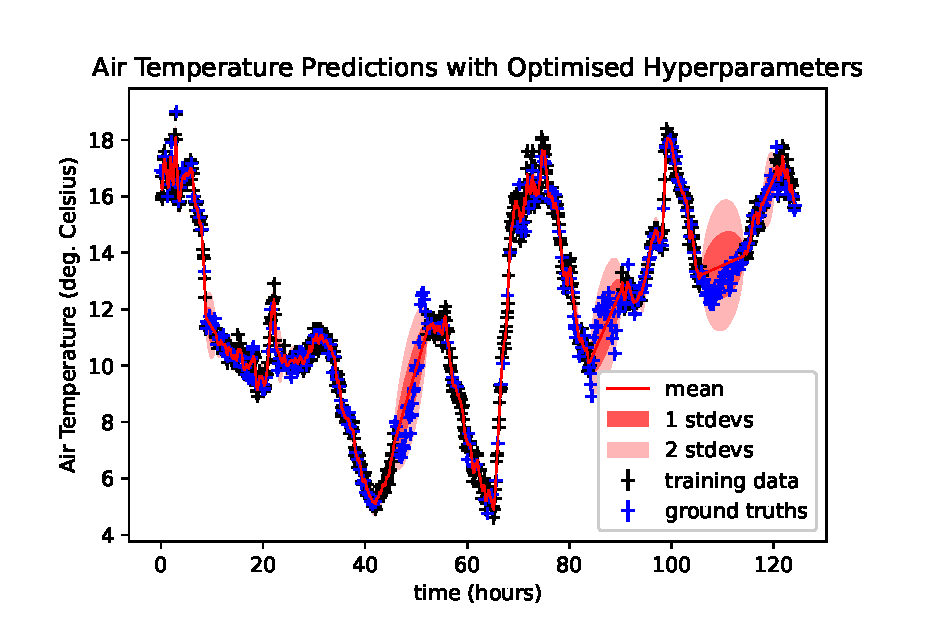
\includegraphics[width=\linewidth,height=\textheight,keepaspectratio]{air_temp_interpolation.eps}
                    \caption{This plot shows the posterior mean function and the standard deviation that the posterior distribution assigns to each point when interpolating missing air temperature measurements. The variance of the posterior distribution increases quickly in the gaps between training datapoints.}
                    \label{plot_airtempinterpolation}
                \end{figure}

            \FloatBarrier
            \subsection{Interpolation of Tide Height}

                Here too I chose a constant prior mean function for simplicity, and here too the optimised value of the constant was very close to the mean value of the complete dataset. Since the tide height is known to have a period of twelve hours, I chose the linear combination of a periodic function and an exponentiated quadratic as prior covariance function; this combination means that the predicted value for the tide height is influenced both by other points shifted by a whole number of periods and also by points close to the point in question. As can be seen in \cref{plot_tideheightinterpolation}, this leads to a very good fit; the variance of the posterior distribution is quite low but this is justified since it fits the ground truth data very well.

                \begin{figure}
                    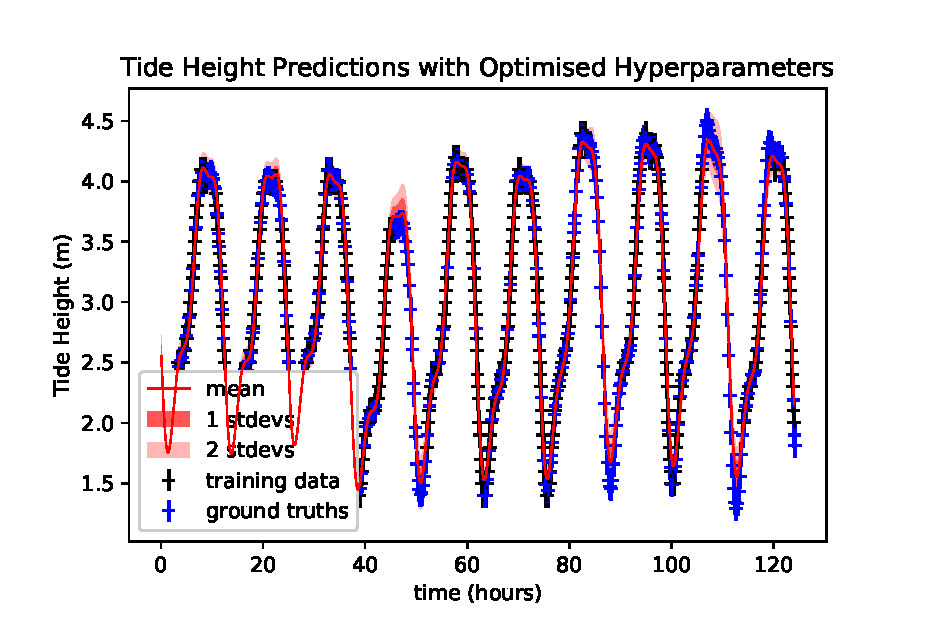
\includegraphics[width=\linewidth,height=\textheight,keepaspectratio]{tide_height_interpolation.eps}
                    \caption{This plot shows the posterior mean function and the standard deviation that the posterior distribution assigns to each point when interpolating missing tide height measurements. The mean function shows a very good fit to the ground truth, so the relatively low variance of the posterior distribution is justified.}
                    \label{plot_tideheightinterpolation}
                \end{figure}

            \FloatBarrier
%    \section{Extrapolation using Gaussian Processes}
%
%            Extrapolating the function outside of the domain of the training data proceeds similarly to the prediction of missing values. The difference is that the posterior distribution is now calculated by conditioning all the datapoints up to a certain time, with the remaining datapoints predicted using the posterior mean function.
%
%            \subsection{Extrapolation of Air Temperature}
%
%
%
%            \subsection{Extrapolation of Tide Height}
%
%                Due to the good performance on the interpolation of the tide height, here too I chose a constant mean function and a linear combination of periodic function and exponentiated quadratic as the covariance function.
%
%                As can be seen in the results in figure %TODO
%                , the model fails to accurately extrapolate when only given the earliest 10\% of readings. These do not cover a whole period, so the training data can be fitted purely by using the exponentiated quadratic term in the covariance function and the periodic term is neglected. When the model is provided with more training data, this issue is alleviated and the model starts to fit the unseen data better. 
%

    \section{Sequential Prediction}
            
            In this section, the predictions and uncertainty for each point were calculated individually using all the training points up to a fixed lookahead before the point in question; the function value at time $t$ is predicted using the training data points up to time $t-\textrm{lookahead}$.

            In implementing this, I used the same mean and covariance functions as in \cref{sec_interpolation} whose hyperparameters were optimised using all available data; while this leads to a better fit to the data than one would expect during actual deployment, it allows us to investigate the effect of varying the lookahead without any confounding effect from bad hyperparameters.

            \subsection{Sequential Prediction of Air Temperature} 

                The Matérn-1/2 covariance function used leads to an excellent fit for small lookahead (\cref{plot_airtemplookahead_5mins}), but as the lookahead gets larger we start to see a more and more pronounced translation of the posterior mean function to the right compared to the ground truth values (\cref{plot_airtemplookahead_30mins} and especially \cref{plot_airtemplookahead_240mins}). This can be explained by the fact that the Matérn-1/2 function is unable to anticipate rapid changes in function value because it is a local covariance function and so assumes that the closest training datapoint has the largest predictive power for the point that the GP is currently trying to predict. If the closest training datapoint is however quite far removed due to a large lookahead, it does not contain any real indication that in the ground truth data a rapid change in function value occurs at the point in question.

                The uncertainty estimates however seem well calibrated and as expected are larger for a larger lookahead and for regions with rapid changes in function value.

                \begin{figure}[ht!]
                    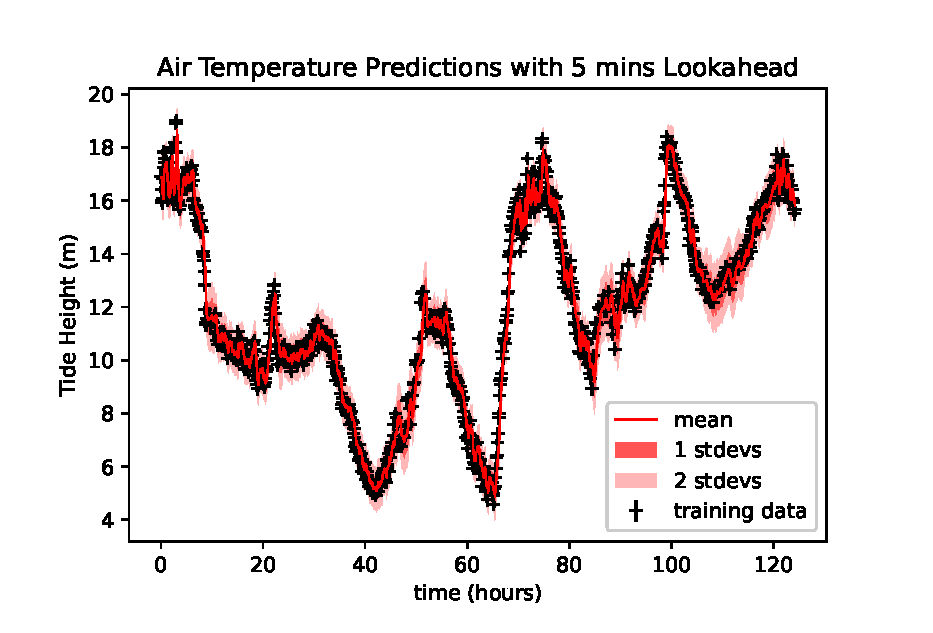
\includegraphics[width=\linewidth,height=\textheight,keepaspectratio]{air_temp_lookahead_5mins.eps}
                    \caption{This plot shows the posterior mean function and the standard deviation that the posterior distribution assigns to each point when predicting air temperature measurements with a lookahead of five minutes. The mean function shows a very good fit to the ground truth but one can already see larger variance in regions with relatively rapid changes in the ground truths.}
                    \label{plot_airtemplookahead_5mins}
                \end{figure}

                \begin{figure}[ht!]
                    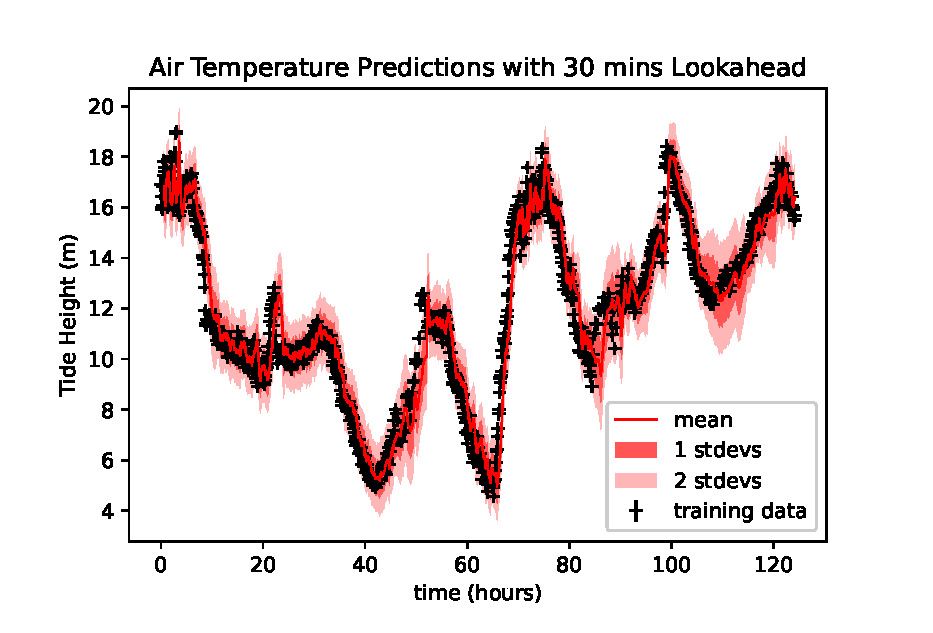
\includegraphics[width=\linewidth,height=\textheight,keepaspectratio]{air_temp_lookahead_30mins.eps}
                    \caption{This plot shows the posterior mean function and the standard deviation that the posterior distribution assigns to each point when predicting air temperature measurements with a lookahead of 30 minutes. The fit of the mean function to the ground truth data is still reasonably good, and the posterior variance has grown to account for the errors that do develop.}
                    \label{plot_airtemplookahead_30mins}
                \end{figure}

                \begin{figure}[ht!]
                    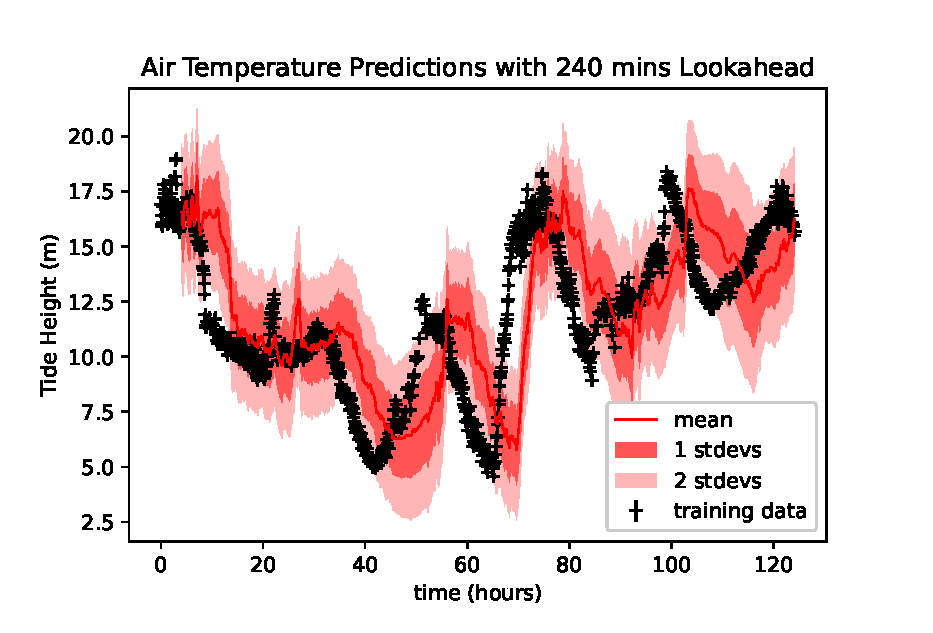
\includegraphics[width=\linewidth,height=\textheight,keepaspectratio]{air_temp_lookahead_240mins.eps}
                    \caption{This plot shows the posterior mean function and the standard deviation that the posterior distribution assigns to each point when predicting air temperature measurements with a lookahead of two hours. One can now very noticeably see that the mean function is translated to the right with respect to the ground truth datapoints.}
                    \label{plot_airtemplookahead_240mins}
                \end{figure}
            
            \FloatBarrier
            \subsection{Sequential Prediction of Tide Height}

                As can be seen in \cref{plot_tideheightlookahead_5mins}, \cref{plot_tideheightlookahead_30mins}, and \cref{plot_tideheightlookahead_240mins}, even for a large lookahead the posterior mean function fits the ground truth data quite well. This is likely a consequence of the very regular and periodic tide height being easy to predict given a well-calibrated covariance function.

                It is noticeable that as the lookahead grows, the uncertainty grows significantly for the first period in particular (compare \cref{plot_tideheightlookahead_5mins} and \cref{plot_tideheightlookahead_30mins}), likely because the GP does not have many training datapoints for the first few datapoints. This is especially pronounced for a large lookahead (\cref{plot_tideheightlookahead_240mins}).
                The GP also has trouble anticipating slightly lower or larger amplitudes when using a large lookahead because it is difficult to anticipate the tide height levelling off earlier than before when the training data barely includes any points from the current period.

                \begin{figure}[ht!]
                    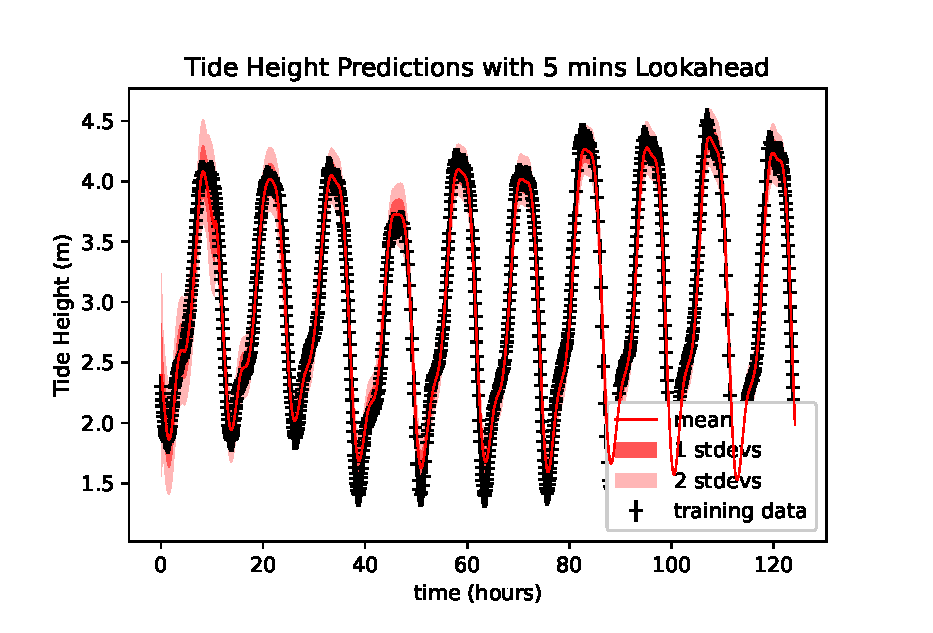
\includegraphics[width=\linewidth,height=\textheight,keepaspectratio]{tide_height_lookahead_5mins.eps}
                    \caption{This plot shows the posterior mean function and the standard deviation that the posterior distribution assigns to each point when predicting tide height measurements with a lookahead of five minutes. The mean function shows a very good fit to the ground truth, with generally small variances.}
                    \label{plot_tideheightlookahead_5mins}
                \end{figure}

                \begin{figure}[ht!]
                    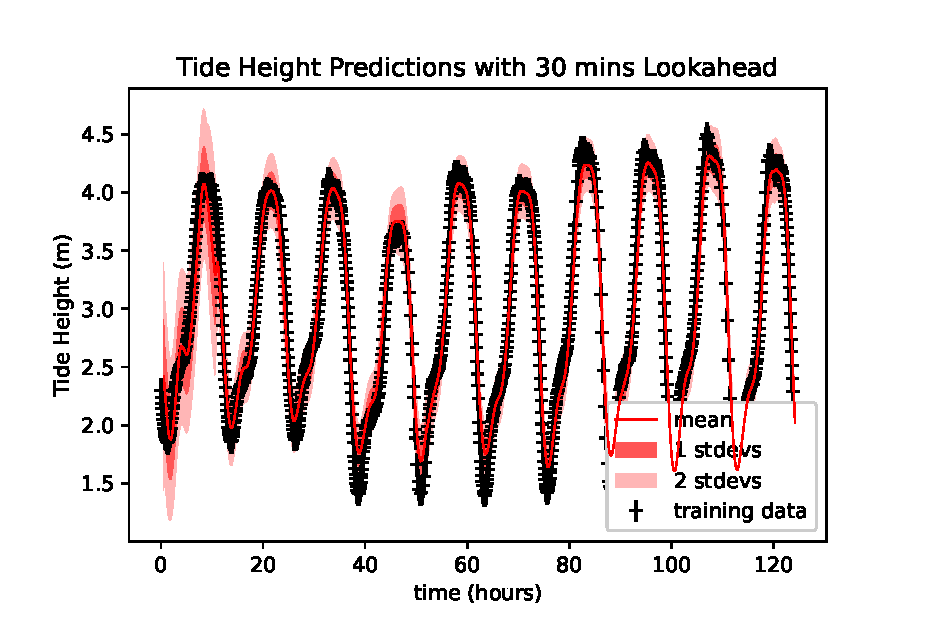
\includegraphics[width=\linewidth,height=\textheight,keepaspectratio]{tide_height_lookahead_30mins.eps}
                    \caption{This plot shows the posterior mean function and the standard deviation that the posterior distribution assigns to each point when predicting tide height measurements with a lookahead of 30 minutes. The fit of the mean function to the ground truth data is still reasonably good but we can see the variances to grow, especially for the first period.}
                    \label{plot_tideheightlookahead_30mins}
                \end{figure}

                \begin{figure}[ht!]
                    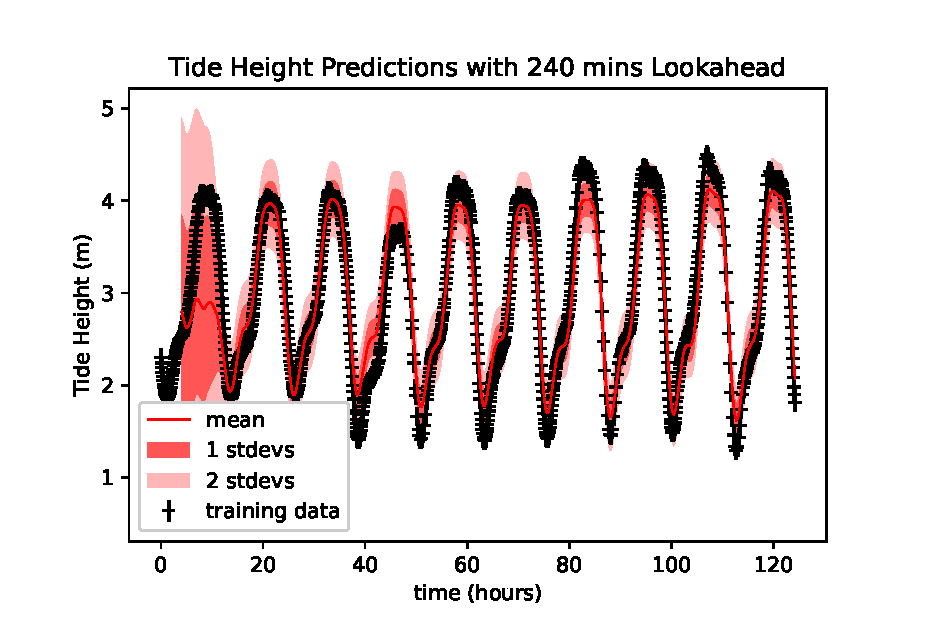
\includegraphics[width=\linewidth,height=\textheight,keepaspectratio]{tide_height_lookahead_240mins.eps}
                    \caption{This plot shows the posterior mean function and the standard deviation that the posterior distribution assigns to each point when predicting tide height measurements with a lookahead of two hours. The mean function still roughly follows the ground truth data, but fails to predict the tide height accurately at the peaks of the plot and especially for the first period where the Gaussian Process only has very few training datapoints to predict the amplitude of the function. This is reflected in much larger posterior variances.}
                    \label{plot_tideheightlookahead_240mins}
                \end{figure}
\end{document}